% Options for packages loaded elsewhere
\PassOptionsToPackage{unicode}{hyperref}
\PassOptionsToPackage{hyphens}{url}
%
\documentclass[
]{book}
\usepackage{lmodern}
\usepackage{amsmath}
\usepackage{ifxetex,ifluatex}
\ifnum 0\ifxetex 1\fi\ifluatex 1\fi=0 % if pdftex
  \usepackage[T1]{fontenc}
  \usepackage[utf8]{inputenc}
  \usepackage{textcomp} % provide euro and other symbols
  \usepackage{amssymb}
\else % if luatex or xetex
  \usepackage{unicode-math}
  \defaultfontfeatures{Scale=MatchLowercase}
  \defaultfontfeatures[\rmfamily]{Ligatures=TeX,Scale=1}
\fi
% Use upquote if available, for straight quotes in verbatim environments
\IfFileExists{upquote.sty}{\usepackage{upquote}}{}
\IfFileExists{microtype.sty}{% use microtype if available
  \usepackage[]{microtype}
  \UseMicrotypeSet[protrusion]{basicmath} % disable protrusion for tt fonts
}{}
\makeatletter
\@ifundefined{KOMAClassName}{% if non-KOMA class
  \IfFileExists{parskip.sty}{%
    \usepackage{parskip}
  }{% else
    \setlength{\parindent}{0pt}
    \setlength{\parskip}{6pt plus 2pt minus 1pt}}
}{% if KOMA class
  \KOMAoptions{parskip=half}}
\makeatother
\usepackage{xcolor}
\IfFileExists{xurl.sty}{\usepackage{xurl}}{} % add URL line breaks if available
\IfFileExists{bookmark.sty}{\usepackage{bookmark}}{\usepackage{hyperref}}
\hypersetup{
  pdftitle={Python for social and experimental psychology},
  pdfauthor={Alexander (Sasha) Pastukhov},
  hidelinks,
  pdfcreator={LaTeX via pandoc}}
\urlstyle{same} % disable monospaced font for URLs
\usepackage{color}
\usepackage{fancyvrb}
\newcommand{\VerbBar}{|}
\newcommand{\VERB}{\Verb[commandchars=\\\{\}]}
\DefineVerbatimEnvironment{Highlighting}{Verbatim}{commandchars=\\\{\}}
% Add ',fontsize=\small' for more characters per line
\usepackage{framed}
\definecolor{shadecolor}{RGB}{248,248,248}
\newenvironment{Shaded}{\begin{snugshade}}{\end{snugshade}}
\newcommand{\AlertTok}[1]{\textcolor[rgb]{0.94,0.16,0.16}{#1}}
\newcommand{\AnnotationTok}[1]{\textcolor[rgb]{0.56,0.35,0.01}{\textbf{\textit{#1}}}}
\newcommand{\AttributeTok}[1]{\textcolor[rgb]{0.77,0.63,0.00}{#1}}
\newcommand{\BaseNTok}[1]{\textcolor[rgb]{0.00,0.00,0.81}{#1}}
\newcommand{\BuiltInTok}[1]{#1}
\newcommand{\CharTok}[1]{\textcolor[rgb]{0.31,0.60,0.02}{#1}}
\newcommand{\CommentTok}[1]{\textcolor[rgb]{0.56,0.35,0.01}{\textit{#1}}}
\newcommand{\CommentVarTok}[1]{\textcolor[rgb]{0.56,0.35,0.01}{\textbf{\textit{#1}}}}
\newcommand{\ConstantTok}[1]{\textcolor[rgb]{0.00,0.00,0.00}{#1}}
\newcommand{\ControlFlowTok}[1]{\textcolor[rgb]{0.13,0.29,0.53}{\textbf{#1}}}
\newcommand{\DataTypeTok}[1]{\textcolor[rgb]{0.13,0.29,0.53}{#1}}
\newcommand{\DecValTok}[1]{\textcolor[rgb]{0.00,0.00,0.81}{#1}}
\newcommand{\DocumentationTok}[1]{\textcolor[rgb]{0.56,0.35,0.01}{\textbf{\textit{#1}}}}
\newcommand{\ErrorTok}[1]{\textcolor[rgb]{0.64,0.00,0.00}{\textbf{#1}}}
\newcommand{\ExtensionTok}[1]{#1}
\newcommand{\FloatTok}[1]{\textcolor[rgb]{0.00,0.00,0.81}{#1}}
\newcommand{\FunctionTok}[1]{\textcolor[rgb]{0.00,0.00,0.00}{#1}}
\newcommand{\ImportTok}[1]{#1}
\newcommand{\InformationTok}[1]{\textcolor[rgb]{0.56,0.35,0.01}{\textbf{\textit{#1}}}}
\newcommand{\KeywordTok}[1]{\textcolor[rgb]{0.13,0.29,0.53}{\textbf{#1}}}
\newcommand{\NormalTok}[1]{#1}
\newcommand{\OperatorTok}[1]{\textcolor[rgb]{0.81,0.36,0.00}{\textbf{#1}}}
\newcommand{\OtherTok}[1]{\textcolor[rgb]{0.56,0.35,0.01}{#1}}
\newcommand{\PreprocessorTok}[1]{\textcolor[rgb]{0.56,0.35,0.01}{\textit{#1}}}
\newcommand{\RegionMarkerTok}[1]{#1}
\newcommand{\SpecialCharTok}[1]{\textcolor[rgb]{0.00,0.00,0.00}{#1}}
\newcommand{\SpecialStringTok}[1]{\textcolor[rgb]{0.31,0.60,0.02}{#1}}
\newcommand{\StringTok}[1]{\textcolor[rgb]{0.31,0.60,0.02}{#1}}
\newcommand{\VariableTok}[1]{\textcolor[rgb]{0.00,0.00,0.00}{#1}}
\newcommand{\VerbatimStringTok}[1]{\textcolor[rgb]{0.31,0.60,0.02}{#1}}
\newcommand{\WarningTok}[1]{\textcolor[rgb]{0.56,0.35,0.01}{\textbf{\textit{#1}}}}
\usepackage{longtable,booktabs}
% Correct order of tables after \paragraph or \subparagraph
\usepackage{etoolbox}
\makeatletter
\patchcmd\longtable{\par}{\if@noskipsec\mbox{}\fi\par}{}{}
\makeatother
% Allow footnotes in longtable head/foot
\IfFileExists{footnotehyper.sty}{\usepackage{footnotehyper}}{\usepackage{footnote}}
\makesavenoteenv{longtable}
\usepackage{graphicx}
\makeatletter
\def\maxwidth{\ifdim\Gin@nat@width>\linewidth\linewidth\else\Gin@nat@width\fi}
\def\maxheight{\ifdim\Gin@nat@height>\textheight\textheight\else\Gin@nat@height\fi}
\makeatother
% Scale images if necessary, so that they will not overflow the page
% margins by default, and it is still possible to overwrite the defaults
% using explicit options in \includegraphics[width, height, ...]{}
\setkeys{Gin}{width=\maxwidth,height=\maxheight,keepaspectratio}
% Set default figure placement to htbp
\makeatletter
\def\fps@figure{htbp}
\makeatother
\setlength{\emergencystretch}{3em} % prevent overfull lines
\providecommand{\tightlist}{%
  \setlength{\itemsep}{0pt}\setlength{\parskip}{0pt}}
\setcounter{secnumdepth}{5}
\usepackage{booktabs}
\ifluatex
  \usepackage{selnolig}  % disable illegal ligatures
\fi
\usepackage[]{natbib}
\bibliographystyle{apalike}

\title{Python for social and experimental psychology}
\author{Alexander (Sasha) Pastukhov}
\date{2020-11-06}

\begin{document}
\maketitle

{
\setcounter{tocdepth}{1}
\tableofcontents
}
\hypertarget{introduction}{%
\chapter*{Introduction}\label{introduction}}
\addcontentsline{toc}{chapter}{Introduction}

\hypertarget{about-the-seminar}{%
\section*{About the seminar}\label{about-the-seminar}}
\addcontentsline{toc}{section}{About the seminar}

This is a material for \emph{Python for social and experimental psychology} seminar. Each chapter covers a single seminar, introducing necessary ideas and is accompanied by a notebook with exercises that you need to complete and submit. The material assumes no foreknowledge of Python or programming from the reader. Its purpose is to gradually build up your knowledge and allow you to create more and more complex games. Yes, games! Of course, the real research is about performing experiments but there is little difference between the two. The basic ingredients are the same and, arguably, experiments are just boring games. And, be assured, if you can program a game, you certainly can program an experiment.

We will start with a simple \emph{Guess a Number} text-only game in which first you and then the computer will be doing the guessing. Next, we will implement a classic \emph{Hunt the Wumpus} text adventure game that will require use of more complex structures. Once we master the basics, we will up the ante by making \emph{video} games with graphics and sounds using \href{https://psychopy.org/}{PsychoPy} library. We will start with a classic \emph{Memory Game} and, then, create a more dynamic game by making a clone of a \emph{Flappy Bird}.

Remember that throughout the seminar you can and should(!) always ask me whenever something is unclear or you do not understand a concept or logic behind certain code. Do not hesitate to write me in the team or (better) directly to me in the chat (in the latter case, the notifications are harder miss and we don't spam others with our conversation).

You will need to submit your assignment one day before the next seminar (Tuesday before noon at the latest), so I would have time evaluate it and provide feedback.

As a final assignment, you will need to program a video game, which will only require the material covered by the seminar. Please inform me, If you require a grade, as then I will create a more specific description for you to have a clear understanding of how the program will be graded.

\hypertarget{note-on-exercises}{%
\section*{Note on exercises}\label{note-on-exercises}}
\addcontentsline{toc}{section}{Note on exercises}

In many exercises your will be not writing the code but reading and understanding it. Your job in this case is ``to think like a computer''. Your advantage is that computers are very dumb, so instructions for them must be written in very simple, clear, and unambiguous way. This means that, with practice, reading code is easy for a human (well, reading a well-written code is easy, you will eventually encounter ``spaghetti-code'' which is easier to rewrite from scratch than to understand). In each case, you simply go line-by-line, doing all computations by hand and writing down values stored in the variables (if there are too many to keep track of). Once you go through code in this manner, it will be completely transparent for you. No mysteries should remain, you should have no doubts or uncertainty about any(!) line. Moreover, then you can run the code and check that the values you are getting from computer match yours. Any difference means you made a mistake and code is working differently from how you think it does. In any case, \textbf{if you not 100\% sure about any line of code, ask me, so we can go through it together!}

In a sense, reading the code is the most important programming skill. It is impossible to learn how to write, if you cannot read first! Moreover, when programming you will probably spend more time reading the code and making sure that it works correctly than writing the new code. Thus, use this opportunity to practice and never use the code that you do not understand completely. This means that you certainly can use \href{https://stackoverflow.com/}{stackoverflow} but do make sure you understand the code you copied!

\hypertarget{why-python}{%
\section*{Why Python?}\label{why-python}}
\addcontentsline{toc}{section}{Why Python?}

The ultimate goal of this seminar is to teach you how to create an experiment for psychology research. There are many ways to achieve this end. You can use drag-and-drop systems either commercial like \href{https://www.neurobs.com/}{Presentation}, \href{https://www.sr-research.com/experiment-builder/}{Experiment Builder} or free like \href{https://psychopy.org/builder}{PsychoPy Bulder interface}. They have a much shallower learning curve, so you can start creating and running your experiments faster. However, the simplicity of their use has a price: They are fairly limited in which stimuli you can use and how you can control the presentation schedule, conditions, feedback, etc. Typically, they allow you to extend them by programming the desired behavior but you do need to know how to program to do this. Thus, I think that while these systems, in particular \href{https://psychopy.org/}{PsychoPy}, are great tools to quickly bang a simple experiment together, they are most useful if you understand how they create the underlying code and how you would program it yourself. Then, you will not be limited by the software, as you know you can program something the default drag-and-drop won't allow, but you can always opt in, if drag-and-drop is sufficient but faster. At the end, it is about having options and creative freedom to program an experiment that will answer your research question, not an experiment that your software allows you to program.

We will learn programming in Python, which is a great language that combines simple and clear syntax with power and ability to tackle almost any problem. The advantage of learning Python, as compared to say Matlab, which is commonly used in neuroscience, is that it allows you do almost anything. In this seminar, we will concentrate on desktop experiments but you can use it for online experiments (\href{https://otree.readthedocs.io/en/latest/}{oTree}), scientific programming (\href{https://numpy.org/}{NumPy} and \href{https://www.scipy.org/}{SciPy}), data analysis (\href{https://pandas.pydata.org/}{pandas}), machine learning (\href{https://keras.io/}{keras}), website programming (\href{https://www.djangoproject.com/}{django}), computer vision (\href{https://opencv.org/}{OpenCV}), etc. Thus, learning Python will give you one of the most versitile programming tools that you can use for all stages of your research or work. And, Python is free, so you do not need to worry whether you or your future employer will be able to afford the license fees (a very real problem, if you use Matlab).

\hypertarget{getting-started}{%
\chapter*{Getting Started}\label{getting-started}}
\addcontentsline{toc}{chapter}{Getting Started}

\hypertarget{install-anaconda}{%
\section*{Installing Anaconda environment}\label{install-anaconda}}
\addcontentsline{toc}{section}{Installing Anaconda environment}

First, install \href{https://www.anaconda.com}{Anaconda}, a Python distribution that includes many packages and tools out-of-the-box, makes it easy to install new packages and keep them updated. Follow this \href{https://www.anaconda.com/products/individual}{link} and download the installer suitable for your platform. You can pick either 32- or 64-bit version. I would recommend the latter, so that we all have maximally similar setup (it won't really make a difference in practice, though). Follow the installer instructions and use defaults, unless you have reasons to modify them (e.g.~folder location, as the drive for the default choice may have limited available space, as in my case).

After installation you will have a new \emph{Anaconda3 (64-bit)} folder that contains links to programs.

\begin{center}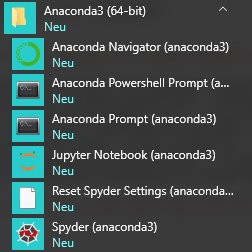
\includegraphics[width=0.5\linewidth]{images/anaconda-shortcuts} \end{center}

You can use \emph{Anaconda Navigator} that allows you to choose a specific programming environment, including \href{https://jupyter.org/}{Jupyter Notebook} that we will use (not JupyterLab, it is more versatile but we want to keep things simple at the beginning!). Alternatively, you can start \emph{Jupyter Notebook} directly from the start menu. Please read the \href{https://jupyter-notebook.readthedocs.io/en/stable/examples/Notebook/examples_index.html}{online documentation} to familiarize yourself with Jupyter Notebook basic interface, e.g.~how to create a new cell, run it, etc.

\hypertarget{install-vs-code}{%
\section*{Installing Visual Studio Code}\label{install-vs-code}}
\addcontentsline{toc}{section}{Installing Visual Studio Code}

\href{https://code.visualstudio.com/}{Visual Studio Code} is a free lightweight open-source editor with strong support for Python. We will start use it in earnest, once our programs grow to be sufficiently long and complex. At the early stages, we will mostly use Jupyter notebooks and I would recommend using Jupyter notebooks using the default browser-based editor you installed as part of \protect\hyperlink{install-anaconda}{Anaconda}. However, you can also work with Jupyter notebooks in VS Code \href{https://code.visualstudio.com/docs/python/jupyter-support}{directly}.

As in case of \protect\hyperlink{install-anaconda}{Anaconda}, download the installer for your platform and follow the instructions. Start VS Code and open any Python file, for example \href{other/empty.py}{this one} (use \texttt{Alt+click} to download it, ignore warnings, it is has only comments, so cannot harm you). When you open Python file for the first time, VS Code will suggest to install a Python extension. Do that and install a linter when VS Code suggests that (\href{https://code.visualstudio.com/docs/python/linting}{linting} highlights syntactical and stylistic problems in your code, making it easier to write consistent clear code).

Once the Python extension is activated, you will see which Python interpreter is used (you can have more than one or you may have multiple \href{https://docs.python.org/3/tutorial/venv.html}{virtual environments}).

\begin{center}
\includegraphics[width=1\linewidth]{images/vscode-python-interpreter} \end{center}

If the selected environment is the wrong one or you are simply not sure, click on it and it will open a drop-down list with all interpreters and environments you have. Consult VS Code \href{https://code.visualstudio.com/docs/python/environments}{online documentation} on environments, if you need to change/add/delete environment (the exact settings may change, so looking at constantly updated online documentation is wiser than copying it here).

\hypertarget{install-psychopy}{%
\section*{Installing PsychoPy}\label{install-psychopy}}
\addcontentsline{toc}{section}{Installing PsychoPy}

This step can wait until the first \protect\hyperlink{memory-game-01}{Memory Game} seminar.

Download and install \href{https://www.psychopy.org/download.html}{Standalone PsychoPy} version. You can install PsychoPy as a conda package or via pip. However, using it as a standalone would ensure that you have all necessary additional libraries and a builder interface for the future use. We will use prepackaged PsychoPy's python environment in \protect\hyperlink{install-vs-code}{VS Code}.

\hypertarget{seminar01}{%
\chapter{Python basics}\label{seminar01}}

Before we start, create a folder called \emph{python-for-experiments} (or with some other more suitable but meaningful name) in you user folder (this is where Anaconda's Jupyter Notebook expects to find them). Download the \href{notebooks/Seminar\%2001.\%20Basics.ipynb}{exercise notebook} and put it in this folder. Open Jupyter Notebook (see \protect\hyperlink{getting-started}{Getting Started}, if you forgot how you do that), navigate to the folder you created and open the downloaded notebook. You will need to switch between explanations here and the exercises in the notebook, so keep them both open.

\hypertarget{variables}{%
\section{Variables}\label{variables}}

The first fundamental concept that we need to be acquainted with is \textbf{variable}. Variables are used to store information and you can think of it as a box with a name tag, so that you can put something into it. The name tag on that box is the name of the variable and its value what you store in it. For example, we can create a variable that stores the number of legs a game character has. We begin with a number typical for a human being.

\begin{center}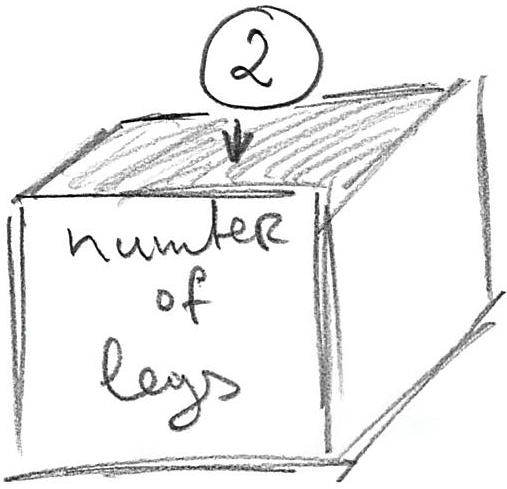
\includegraphics[width=0.5\linewidth]{images/variable-as-box} \end{center}

In Python, you would write

\begin{Shaded}
\begin{Highlighting}[]
\NormalTok{number\_of\_legs }\OperatorTok{=} \DecValTok{2}
\end{Highlighting}
\end{Shaded}

The \textbf{assignment statement} above has very simple structure \texttt{\textless{}variable-name\textgreater{}\ =\ \textless{}value\textgreater{}}. Variable name (name tag on the box) should be meaningful, it can start with letters or \_ and can contain letters, numbers, and \_ symbol but not spaces, tabs, special characters, etc. Python recommends (well, actually, \href{https://www.python.org/dev/peps/pep-0008/}{insists}) that you use \textbf{snake\_case} (all lower-case, underscore for spaces) to format your variable names. The \texttt{\textless{}value\textgreater{}} on the right side is a more complex story, as it can be hard-coded (as in example above), computed using other variables or the same variable, returned by a function, etc.

Using variables means that you can concentrate what corresponding values \textbf{mean} rather than worrying about what these values are. For example, the next time you need to compute something based on number of character's legs (e.g., how many pairs of shoes does a character need), you can compute it based on current value of \texttt{number\_of\_legs} variable rather than assume that it is \texttt{1}.

\begin{Shaded}
\begin{Highlighting}[]
\CommentTok{\# BAD: why 1? Is it because the character has two legs or}
\CommentTok{\# because we issue one pair of shoes per character irrespective of}
\CommentTok{\# their actual number of legs?}
\NormalTok{pairs\_of\_shoes }\OperatorTok{=} \DecValTok{1}

\CommentTok{\# BETTER!}
\NormalTok{pairs\_of\_shoes }\OperatorTok{=}\NormalTok{ number\_of\_legs }\OperatorTok{/} \DecValTok{2}
\end{Highlighting}
\end{Shaded}

Variables also give you flexibility. Their values can change during the program run: player's score is increasing, number of lives decreasing, number of spells it can cast grows or falls depending on their use, etc. Yet, you can always use the value in the variable to perform necessary computations. For example, here is a slightly extended \texttt{number\_of\_shoes} example.

\begin{Shaded}
\begin{Highlighting}[]
\NormalTok{number\_of\_legs }\OperatorTok{=} \DecValTok{2}

\CommentTok{\# ...}
\CommentTok{\# something happens and our character is turned into an octopus}
\NormalTok{number\_of\_legs }\OperatorTok{=} \DecValTok{8}
\CommentTok{\# ...}

\CommentTok{\# the same code still works and we still can compute the correct number of pairs of shoes}
\NormalTok{pairs\_of\_shoes }\OperatorTok{=}\NormalTok{ number\_of\_legs }\OperatorTok{/} \DecValTok{2}
\end{Highlighting}
\end{Shaded}

As noted above, you can think about a variable as a labeled box you can store something in. That means that you can always ``throw away'' the old value and put something new. In case of variables, the ``throwing away'' part happens automatically, as the new value overwrites the old one. Check yourself, what will be final value of the variable in the code below?

\begin{Shaded}
\begin{Highlighting}[]
\NormalTok{number\_of\_legs }\OperatorTok{=} \DecValTok{2}
\NormalTok{number\_of\_legs }\OperatorTok{=} \DecValTok{5}
\NormalTok{number\_of\_legs }\OperatorTok{=} \DecValTok{1}
\NormalTok{number\_of\_legs}
\end{Highlighting}
\end{Shaded}

Do exercise \#1.

As you have already seen, you can \emph{compute} a value instead of specifying it. What would be the answer here?

\begin{Shaded}
\begin{Highlighting}[]
\NormalTok{number\_of\_legs }\OperatorTok{=} \DecValTok{2} \OperatorTok{*} \DecValTok{2}
\NormalTok{number\_of\_legs }\OperatorTok{=} \DecValTok{7} \OperatorTok{{-}} \DecValTok{2}
\NormalTok{number\_of\_legs}
\end{Highlighting}
\end{Shaded}

Do exercise \#2.

\hypertarget{assignments-are-not-equations}{%
\section{Assignments are not equations!}\label{assignments-are-not-equations}}

\textbf{Very important}: although assignments \emph{look} like mathematical equations, they are \textbf{not equations!} Assignments follow a \textbf{very important} rule that you must keep in mind when understanding assignments: the right side expression is evaluated \emph{first} until the final value is computed, then and only then the final value is assigned to the variable specified on the left side (put in the box). What this means is that you can use the same variable on \emph{both} sides! Let's take a look at this code:

\begin{Shaded}
\begin{Highlighting}[]
\NormalTok{x }\OperatorTok{=} \DecValTok{2}
\NormalTok{y }\OperatorTok{=} \DecValTok{5}
\NormalTok{x }\OperatorTok{=}\NormalTok{ x }\OperatorTok{+}\NormalTok{ y }\OperatorTok{{-}} \DecValTok{4}
\end{Highlighting}
\end{Shaded}

What happens when computer evaluates the last line?

\begin{Shaded}
\begin{Highlighting}[]
\NormalTok{x }\OperatorTok{=}\NormalTok{ x }\OperatorTok{+}\NormalTok{ y }\OperatorTok{{-}} \DecValTok{4}
\end{Highlighting}
\end{Shaded}

First, it takes \emph{current} values of all variables (\texttt{2} for \texttt{x} and \texttt{5} for \texttt{y}) and substitutes them into the expression. After that internal step, the expression looks like

\begin{Shaded}
\begin{Highlighting}[]
\NormalTok{x }\OperatorTok{=} \DecValTok{2} \OperatorTok{+} \DecValTok{5} \OperatorTok{{-}} \DecValTok{4}
\end{Highlighting}
\end{Shaded}

Then, it computes the expression on the right side and, \textbf{once the computation is completed}, stores that new value in \texttt{x}

\begin{Shaded}
\begin{Highlighting}[]
\NormalTok{x }\OperatorTok{=} \DecValTok{3}
\end{Highlighting}
\end{Shaded}

Do exercise \#3 to make sure you understand this.

\hypertarget{constants}{%
\section{Constants}\label{constants}}

Although the real power of variables is that you can change their value, you should use them even if the value remains constant. There are no true constants in Python, rather an agreement that their names should be all \texttt{UPPER\_CASE}. Accordingly, when you see \texttt{SUCH\_A\_VARIABLE} you know that you should not change its value. Technically, this is just a recommendation, as no one can stop you from modifying value of a \texttt{CONSTANT}. However, much of Python's ease-of-use comes from such ``gentlemen's agreements'' (such as \texttt{snake\_case} convention above), which you should respect. We will encounter more of them when learning about objects.

Taking all this into account, if number of legs stays constant throughout the game, you should highlight that constancy and write

\begin{Shaded}
\begin{Highlighting}[]
\NormalTok{NUMBER\_OF\_LEGS }\OperatorTok{=} \DecValTok{2}
\end{Highlighting}
\end{Shaded}

I strongly recommend using constants and avoid hardcoding the values. First, if you have several identical values that mean different things (2 legs, 2 eyes, 2 ears, 2 vehicles per character, etc.), seeing a \texttt{2} in the code will not tell you what does this \texttt{2} mean (the legs? the ears? the score multiplier?). You can, of course, figure it out based on the code that uses this number but you could spare yourself that extra effort and use a constant instead. Then, you just read its name and the meaning of the value becomes apparent (and it is the meaning not the actual value that you are mostly interested in). Second, if you decide to \emph{change} that value (say, our main character is now a tripod), when using a constant means you have only one place to worry about, the rest of the code stays as is. If you hard-coded that number, you are in for an exciting (not really) but definitely long search-and-replace throughout the entire code.

Do exercise \#4.

\hypertarget{value-types}{%
\section{Value types}\label{value-types}}

So far, we only used integer numeric values (1, 2, 5, 1000\ldots). Although, Python supports \href{https://docs.python.org/3/library/stdtypes.html}{many different value types}, at first we will concentrate on a small subset of them:

\begin{itemize}
\tightlist
\item
  integer numbers, we already used, e.g.~\texttt{-1}, \texttt{100000}, \texttt{42}.
\item
  float numbers that can take any real value, e.g.~\texttt{42.0}, \texttt{3.14159265359}, \texttt{2.71828}.
\item
  strings that can store text. The text is enclosed between either paired quotes \texttt{"some\ text"} or apostrophes \texttt{\textquotesingle{}some\ text\textquotesingle{}}. This means that you can use quotes or apostrophes inside the string, as long as its is enclosed by the alternative. E.g., \texttt{"students\textquotesingle{}\ homework"} (enclosed in \texttt{"}, apostrophe \texttt{\textquotesingle{}} inside) or \texttt{\textquotesingle{}"All\ generalizations\ are\ false,\ including\ this\ one."\ Mark\ Twain\textquotesingle{}} (quotation enclosed by apostrophes). There is much much more to strings and we will cover that material throughout the course.
\item
  logical / Boolean values that are either \texttt{True} or \texttt{False}.
\end{itemize}

When using a variable it is important that you know what type of value it stores and this is mostly on you. Python will raise an error, if you try doing a computation using incompatible. In some cases, Python will automatically convert values between certain types, e.g.~any integer value is also a real value, so conversion from \texttt{1} to \texttt{1.0} is mostly trivial and automatic. However, in other cases you may need to use explicit conversion. Go to exercise \#5 and try guessing which code will run and which will throw an error due to incompatible types?

\begin{Shaded}
\begin{Highlighting}[]
\DecValTok{5} \OperatorTok{+} \FloatTok{2.0}
\CommentTok{\textquotesingle{}5\textquotesingle{}} \OperatorTok{+} \DecValTok{2}
\CommentTok{\textquotesingle{}5\textquotesingle{}} \OperatorTok{+} \StringTok{\textquotesingle{}2\textquotesingle{}}
\CommentTok{\textquotesingle{}5\textquotesingle{}} \OperatorTok{+} \VariableTok{True}
\DecValTok{5} \OperatorTok{+} \VariableTok{True}
\end{Highlighting}
\end{Shaded}

Do exercise \#5.

Surprised by the last one? This is because internally, \texttt{True} is also \texttt{1} and \texttt{False} is \texttt{0}!

You can explicitly convert from one type to another using special functions. For example, to turn a number or a logical value into a string, you simply write \texttt{str(\textless{}value\textgreater{})}. In examples below, what would be the result?

\begin{Shaded}
\begin{Highlighting}[]
\BuiltInTok{str}\NormalTok{(}\DecValTok{10} \OperatorTok{/} \DecValTok{2}\NormalTok{)}
\BuiltInTok{str}\NormalTok{(}\FloatTok{2.5} \OperatorTok{+} \VariableTok{True}\NormalTok{)}
\BuiltInTok{str}\NormalTok{(}\VariableTok{True}\NormalTok{)}
\end{Highlighting}
\end{Shaded}

Do exercise \#6.

Similarly, you can convert to a logical/Boolean variable using \texttt{bool(\textless{}value\textgreater{})} function. The rules are simple, for numeric values \texttt{0} is \texttt{False}, any other non-zero value is converted to \texttt{True}. For string, an empty string \texttt{\textquotesingle{}\textquotesingle{}} is evaluated to \texttt{False} and non-empty string is converted to \texttt{True}. What would be the output in the examples below?

\begin{Shaded}
\begin{Highlighting}[]
\BuiltInTok{bool}\NormalTok{(}\OperatorTok{{-}}\DecValTok{10}\NormalTok{)}
\BuiltInTok{bool}\NormalTok{(}\FloatTok{0.0}\NormalTok{)}

\NormalTok{secret\_message }\OperatorTok{=} \StringTok{\textquotesingle{}\textquotesingle{}}
\BuiltInTok{bool}\NormalTok{(secret\_message)}

\BuiltInTok{bool}\NormalTok{(}\StringTok{\textquotesingle{}False\textquotesingle{}}\NormalTok{)}
\end{Highlighting}
\end{Shaded}

Do exercise \#7.

Converting to integer or float numbers is trickier. The simplest case is from logical to integer/float, as \texttt{True} gives you \texttt{int(True)} is \texttt{1} and \texttt{float(True)} is \texttt{1.0} and \texttt{False} gives you \texttt{0}/\texttt{0.0}. When converting from float to integer, Python simply drops the fractional part (not rounding!). When converting a string, it must be a valid number of the corresponding type or the error is generated. E.g., you can convert a string like \texttt{"123"} to and integer or a float but this won't work for \texttt{"a123"}. Moreover, you can convert \texttt{"123.4"} to floating-point number but not to an integer, as it has fractional part in it. Given all this, which cells would work and what output would they produce?

\begin{Shaded}
\begin{Highlighting}[]
\BuiltInTok{float}\NormalTok{(}\VariableTok{False}\NormalTok{)}
\BuiltInTok{int}\NormalTok{(}\OperatorTok{{-}}\FloatTok{3.3}\NormalTok{)}
\BuiltInTok{float}\NormalTok{(}\StringTok{"67.8"}\NormalTok{)}
\BuiltInTok{int}\NormalTok{(}\StringTok{"123+3"}\NormalTok{)}
\end{Highlighting}
\end{Shaded}

Do exercise \#8.

\hypertarget{printing-output}{%
\section{Printing output}\label{printing-output}}

To print the value, you need you use \texttt{print()} function (we will talk about functions in general later). In the simplest case, you pass the value and it will be printed out.

\begin{Shaded}
\begin{Highlighting}[]
\BuiltInTok{print}\NormalTok{(}\DecValTok{5}\NormalTok{)}
\end{Highlighting}
\end{Shaded}

\begin{verbatim}
## 5
\end{verbatim}

or

\begin{Shaded}
\begin{Highlighting}[]
\BuiltInTok{print}\NormalTok{(}\StringTok{"five"}\NormalTok{)}
\end{Highlighting}
\end{Shaded}

\begin{verbatim}
## five
\end{verbatim}

Of course, you already know about the variables, so rather than putting a value directly, you can pass a variable instead and its value will be printed out.

\begin{Shaded}
\begin{Highlighting}[]
\NormalTok{number\_of\_pancakes }\OperatorTok{=} \DecValTok{10}
\BuiltInTok{print}\NormalTok{(number\_of\_pancakes)}
\end{Highlighting}
\end{Shaded}

\begin{verbatim}
## 10
\end{verbatim}

or

\begin{Shaded}
\begin{Highlighting}[]
\NormalTok{breakfast }\OperatorTok{=} \StringTok{"pancakes"}
\BuiltInTok{print}\NormalTok{(breakfast)}
\end{Highlighting}
\end{Shaded}

\begin{verbatim}
## pancakes
\end{verbatim}

You can also pass more than one value/variable to the print function and all the values will be printed one after another. For example, if we want to tell the user what did I had for breakfast and just how many of those, we can do

\begin{Shaded}
\begin{Highlighting}[]
\NormalTok{breakfast }\OperatorTok{=} \StringTok{"pancakes"}
\NormalTok{number\_of\_items }\OperatorTok{=} \DecValTok{10}
\BuiltInTok{print}\NormalTok{(breakfast, number\_of\_items)}
\end{Highlighting}
\end{Shaded}

\begin{verbatim}
## pancakes 10
\end{verbatim}

What will be printed by the code below?

\begin{Shaded}
\begin{Highlighting}[]
\NormalTok{dinner }\OperatorTok{=} \StringTok{"stake"}
\NormalTok{count }\OperatorTok{=} \DecValTok{4}
\NormalTok{desert }\OperatorTok{=} \StringTok{"cupcakes"}

\BuiltInTok{print}\NormalTok{(count, dinner, count, desert)}
\end{Highlighting}
\end{Shaded}

Do exercise \#9.

However, you probably would want to be more explicit, when you print out the information. For example, imagine you have these three variables:

\begin{Shaded}
\begin{Highlighting}[]
\NormalTok{meal }\OperatorTok{=} \StringTok{"breakfast"}
\NormalTok{dish }\OperatorTok{=} \StringTok{"pancakes"}
\NormalTok{count }\OperatorTok{=} \DecValTok{10}
\end{Highlighting}
\end{Shaded}

You could, of course do \texttt{print(meal,\ dish,\ count)} but it would be nicer to print ``\emph{I had \textbf{10 pancakes} for \textbf{breakfast}}'', where items in bold would be the inserted variables' values. For this, we need to use string formatting. Please note that the string formatting is not specific to printing, you can create a new string value via formatting and store it in a variable (without printing it out) or print it out (without storing it).

\hypertarget{string-formatting}{%
\section{String formatting}\label{string-formatting}}

A great resource on string formatting in Python is \href{https://pyformat.info/}{pyformat.info}. As Python constantly evolves, it now has more than one way to format strings. Below, I will introduce the ``old'' format that is based on classic string formatting used in \texttt{sprintf} function is C, Matlab, R, and many other programming languages. It is somewhat less flexible than a newer ones but for simple tasks the difference is negligible. Knowing the old format is useful because of its generality. If you want to learn alternatives, read at the link above.

The general call is \texttt{"a\ string\ with\ formatting"\%(tuple\ of\ values\ to\ be\ used\ during\ formatting)}.

In \texttt{"a\ string\ with\ formatting"}, you specify where you want to put the value via \texttt{\%} symbol that is followed by an \emph{optional} formatting info and the \emph{required} symbol that defines the \textbf{type} of the value. The type symbols are

\begin{itemize}
\tightlist
\item
  \texttt{s} for string
\item
  \texttt{d} for an integer
\item
  \texttt{f} for a float value
\item
  \texttt{g} for an ``optimally'' printed float value, so that scientific notation is used for large values (\emph{e.g.}, \texttt{10e5} instead of \texttt{100000}).
\end{itemize}

Here is an example of formatting a string using an integer:

\begin{Shaded}
\begin{Highlighting}[]
\BuiltInTok{print}\NormalTok{(}\StringTok{"I had }\SpecialCharTok{\%d}\StringTok{ pancakes for breakfast"}\OperatorTok{\%}\NormalTok{(}\DecValTok{10}\NormalTok{))}
\end{Highlighting}
\end{Shaded}

\begin{verbatim}
## I had 10 pancakes for breakfast
\end{verbatim}

You are not limited to a single value that you can put into a string. You can specify more locations via \texttt{\%} but you must make sure that you pass the right number of values. Before running it, can you figure out which call will actually work (and what will be the output ) and which will produce an error?

\begin{Shaded}
\begin{Highlighting}[]
\BuiltInTok{print}\NormalTok{(}\StringTok{\textquotesingle{}I had }\SpecialCharTok{\%d}\StringTok{ pancakes and either }\SpecialCharTok{\%d}\StringTok{  or }\SpecialCharTok{\%d}\StringTok{ stakes for dinner\textquotesingle{}}\OperatorTok{\%}\NormalTok{(}\DecValTok{2}\NormalTok{))}
\BuiltInTok{print}\NormalTok{(}\StringTok{\textquotesingle{}I had }\SpecialCharTok{\%d}\StringTok{ pancakes and }\SpecialCharTok{\%d}\StringTok{ stakes for dinner\textquotesingle{}}\OperatorTok{\%}\NormalTok{(}\DecValTok{7}\NormalTok{, }\DecValTok{10}\NormalTok{))}
\BuiltInTok{print}\NormalTok{(}\StringTok{\textquotesingle{}I had }\SpecialCharTok{\%d}\StringTok{ pancakes and }\SpecialCharTok{\%d}\StringTok{ stakes for dinner\textquotesingle{}}\OperatorTok{\%}\NormalTok{(}\DecValTok{1}\NormalTok{, }\DecValTok{7}\NormalTok{, }\DecValTok{10}\NormalTok{))}
\end{Highlighting}
\end{Shaded}

Do exercise \#10.

In case of real values you have two options: \texttt{\%f} and \texttt{\%g}. The latter uses scientific notation (e.g.~\texttt{1e10} for \texttt{10000000000}) to make a representation more compact.

Do exercise \#11 to get a better feeling for the difference.

These is much more to formatting and you can read about it at \href{https://pyformat.info/}{pyformat.info}. However, these basics are sufficient for us to start programming our first game during the next seminar. Don't forget to submit your exercise notebook and see you next time!

\hypertarget{seminar02}{%
\chapter{Guess the Number}\label{seminar02}}

Seminar \#1 covered Python basics, so now you are ready to start developing you first game! We will build it step by step and there will be a lot to learn about input, libraries, conditional statements, and indentation. As before, download \href{notebooks/Seminar\%2002.\%20Guess\%20the\%20number.ipynb}{exercise notebook}, copy it in your designated folder, and open it in Jupyter Notebook.

\hypertarget{game-description}{%
\section{Game description}\label{game-description}}

We will program a game in which one participant (computer) picks the number within a certain range (say, between 1 and 10) and the other participant (player) is trying to guess it. After every guess, the first participant (computer) responds whether the actual number is lower than a guess, higher than a guess, or matches it. The game is over when the player correctly guess the number or (in the later version of the game) runs out of attempts.

Our first version will allow just one attempt (will make it more fun later on) and the overall game algorithm will look like this:

\begin{Shaded}
\begin{Highlighting}[]
\CommentTok{\# 1. computer generates a random number}
\CommentTok{\# 2. prints it out for debug purposes}
\CommentTok{\# 3. prompts user to enter a guess}
\CommentTok{\# 4. compares two numbers and print outs the outcome}
\CommentTok{\#    "My number is lower", "My number is higher", or "Spot on!"}
\end{Highlighting}
\end{Shaded}

\hypertarget{lets-pick-the-number-exercise-1}{%
\section{Let's pick the number (Exercise 1)}\label{lets-pick-the-number-exercise-1}}

Let us start by creating a variable that will hold a number that computer ``picked''. Let us name it \texttt{number\_picked} (you can some other meaningful name as well but it might be easier if we all stick to the same name). To make things a bit simpler at the beginning, let us assign some hard=coded arbitrary number between 1 and 10 to it (whatever you fill like). Then, let us print it out, so that we know the number ourselves (we know it now but that won't be the case when computer will generate it randomly). Use string formatting to make things user-friendly, e.g., print out something like ``The number I've picked is \ldots{}''. Your code should be a two-liner:

\begin{Shaded}
\begin{Highlighting}[]
\CommentTok{\# 1. create variable and set it value}
\CommentTok{\# 2. print out the value}
\end{Highlighting}
\end{Shaded}

Put your code into exercise \#1 and make sure your code works!.

\hypertarget{input-function}{%
\section{Asking user for a guess (Exercise 2)}\label{input-function}}

Now we need to ask the player to enter their guess. For this, we will use \href{https://docs.python.org/3/library/functions.html\#input}{input({[}prompt{]})} function (here and below the links lead to the official documentation). It prints out \texttt{prompt} (a string) if you supplied it, reads the input (key presses) until the user presses \texttt{Enter}, and returns it \textbf{as a string}. For a moment, let us assume that the input is always an valid integer number (so, type only valid integers!), so we can convert it to an integer without extra checks (will add them later) and assign this value to a new variable called \texttt{guess}. Thus, you need to write a single line assignment statement with \texttt{guess} variable on the left side, whereas on the right should be a call to the \texttt{input(...)} function (think of a nice prompt message) wrapped by the type-conversion to \texttt{int(...)}. Switch to exercise 2 and, for the moment, only enter valid integers when running the code, so that the conversion works without an error.

Put your code into exercise \#2.

\hypertarget{conditional-if-statement}{%
\section{\texorpdfstring{Conditional \emph{if} statement}{Conditional if statement}}\label{conditional-if-statement}}

Now we have two numbers: One that computer picked and one that is player's guess. Now, we need to compare them to provide correct output message. For this, we will use conditional \href{https://docs.python.org/3/tutorial/controlflow.html\#if-statements}{if statement}:

\begin{Shaded}
\begin{Highlighting}[]
\ControlFlowTok{if}\NormalTok{ some\_condition\_is\_true:}
    \CommentTok{\# do something}
\ControlFlowTok{elif}\NormalTok{ some\_other\_condition\_is\_true:}
    \CommentTok{\# do something else}
\ControlFlowTok{elif}\NormalTok{ yet\_another\_condition\_is\_true:}
    \CommentTok{\# do yet something else}
\ControlFlowTok{else}\NormalTok{:}
    \CommentTok{\# do something only if all conditions above are false.}
\end{Highlighting}
\end{Shaded}

Only the \texttt{if} part is required, whereas \texttt{elif} (short for ``else, if'') and \texttt{else} are optional. Thus you can do something, only if a condition is true:

\begin{Shaded}
\begin{Highlighting}[]
\ControlFlowTok{if}\NormalTok{ some\_condition\_is\_true:}
    \CommentTok{\# do something, but OTHERWISE DO NOT DO ANYTHING }
    \CommentTok{\# and continue with code execution}
  
\CommentTok{\# some code that is executed after the if{-}statement,}
\CommentTok{\# irrespective of whether the condition was true or not.}
\end{Highlighting}
\end{Shaded}

Before we can properly use conditional statements, you need to understand (1) the conditions themselves and (2) use of indentation as a mean of grouping statements together.

\hypertarget{conditions-and-comparisons-exercises-3-8}{%
\section{Conditions and comparisons (exercises 3-8)}\label{conditions-and-comparisons-exercises-3-8}}

Condition is any expression that can be evaluated to see whether it is \texttt{True} or \texttt{False}. A straightforward example of such expression are comparisons, in human language expressed as ``is today Thursday?'', ``is the answer equal to 42'', ``is it raining and I have an umbrella?''. We will concentrate on them here but later you will see that in Python \textbf{any} expression is either \texttt{True} or \texttt{False}, even when it does not look like a comparison.

For the comparison, you can use the following operators:

\begin{itemize}
\tightlist
\item
  \emph{``A is equal B''} is written as \texttt{A\ ==\ B}.
\item
  \emph{``A is not equal B''} is written as \texttt{A\ !=\ B}.
\item
  \emph{``A is greater than B''} and \emph{``A is smaller than B''} are, respectively, \texttt{A\ \textgreater{}\ B} and \texttt{A\ \textless{}\ B}.
\item
  \emph{``A is greater than or equal to B''} and \emph{``A is smaller than or equal to B''} are, respectively, \texttt{A\ \textgreater{}=\ B} and \texttt{A\ \textless{}=\ B} (please note the order of symbols!).
\end{itemize}

Go to exercise \#3 to solve some comparisons.

You can \emph{invert} the logical value using \texttt{not} operator, as \texttt{not\ True} is \texttt{False} and \texttt{not\ False} is \texttt{True}. This means that \texttt{A\ !=\ B} is the same as \texttt{not\ A\ ==\ B} and, correspondingly, \texttt{A\ ==\ B} is \texttt{not\ A\ !=\ B}. To see how that works, consider both cases when \texttt{A} is indeed equal \texttt{B} and when it is not.

\begin{itemize}
\tightlist
\item
  If A is equal B then \texttt{A\ ==\ B} evaluates to \texttt{True}. The \texttt{A\ !=\ B} is then \texttt{False}, so \texttt{not\ A\ !=\ B} → \texttt{not\ False} → \texttt{True}.
\item
  If A is not equal B then \texttt{A\ ==\ B} evaluates to \texttt{False}. The \texttt{A\ !=\ B} is then \texttt{True}, so \texttt{not\ A\ !=\ B} → \texttt{not\ True} → \texttt{False}.
\end{itemize}

Go to exercise \#4 to explore this inversion yourself.

You can also combine several comparisons using \texttt{and} and/or \texttt{or} operators. As in human language, \texttt{and} means that both parts must be true: \texttt{True\ and\ True} → \texttt{True} but \texttt{True\ and\ False} → \texttt{False}, \texttt{False\ and\ True} → \texttt{False}, and \texttt{False\ and\ False} → \texttt{False}. Same holds if you have more have than two conditions/comparisons, \textbf{all} of them must be true. In case of \texttt{or} only one of the statements must be true, e.g.~\texttt{True\ and\ True} → \texttt{True}, \texttt{True\ and\ False} → \texttt{True}, \texttt{False\ and\ True} → \texttt{True}, but \texttt{False\ and\ False} → \texttt{False}. Again, for more than two comparisons/conditions at least one of them should be true for the entire expression to be true.

Do exercises \#5 and \#6.

Subtle but important point: conditions are evaluated from left to right until the whole expression can be definitely resolved. This means that if the first expression in a \texttt{and} pair is \texttt{False}, the second one is \textbf{never evaluated}. I.e., if \texttt{first\ and\ second} expressions both need to be \texttt{True} and you know that already \texttt{first} expression is false, the whole expression will be \texttt{False} in any case. This means that in the code below there will be no error, even though evaluating \texttt{int("e123")} raises \texttt{ValueError}.

\begin{Shaded}
\begin{Highlighting}[]
\DecValTok{2} \OperatorTok{*} \DecValTok{2} \OperatorTok{==} \DecValTok{5} \KeywordTok{and} \BuiltInTok{int}\NormalTok{(}\StringTok{"e123"}\NormalTok{) }\OperatorTok{==} \DecValTok{123}
\end{Highlighting}
\end{Shaded}

However, reverse the order, so that \texttt{int("e123")\ ==\ 123} needs to be evaluated first and you get the error message

\begin{Shaded}
\begin{Highlighting}[]
\BuiltInTok{int}\NormalTok{(}\StringTok{"e123"}\NormalTok{) }\OperatorTok{==} \DecValTok{123} \KeywordTok{and} \DecValTok{2} \OperatorTok{*} \DecValTok{2} \OperatorTok{==} \DecValTok{4}
\CommentTok{\# Generates ValueError: invalid literal for int() with base 10: \textquotesingle{}e123\textquotesingle{}}
\end{Highlighting}
\end{Shaded}

Similarly, if \emph{any} expression in \texttt{or} is \texttt{True}, you do not need to check the rest.

\begin{Shaded}
\begin{Highlighting}[]
\DecValTok{2} \OperatorTok{*} \DecValTok{2} \OperatorTok{==} \DecValTok{4} \KeywordTok{or} \BuiltInTok{int}\NormalTok{(}\StringTok{"e123"}\NormalTok{) }\OperatorTok{==} \DecValTok{123}
\end{Highlighting}
\end{Shaded}

However, if the first condition is \texttt{False}, we do need to continue (and stumble into an error):

\begin{Shaded}
\begin{Highlighting}[]
\DecValTok{2} \OperatorTok{*} \DecValTok{2} \OperatorTok{==} \DecValTok{5} \KeywordTok{or} \BuiltInTok{int}\NormalTok{(}\StringTok{"e123"}\NormalTok{) }\OperatorTok{==} \DecValTok{123}
\CommentTok{\# Generates ValueError: invalid literal for int() with base 10: \textquotesingle{}e123\textquotesingle{}}
\end{Highlighting}
\end{Shaded}

Do exercise \#7.

Finally, like in simple arithmetic, you can use brackets \texttt{()} to group conditions together. Thus a statement ``I always eat chocolate but I eat spinach only when I am hungry'' can be written as \texttt{food\ ==\ "chocolate"\ or\ (food\ ==\ "spinach"\ and\ hungry)}. Here, \texttt{the\ food\ ==\ "chocolate"} and \texttt{food\ ==\ "spinach"\ and\ hungry} are evaluated independently, their values are substituted in their place and then the \texttt{and} condition is evaluated.

Do exercise \#8.

\hypertarget{grouping-statements-via-identation-exercise-9}{%
\section{Grouping statements via identation (exercise \#9)}\label{grouping-statements-via-identation-exercise-9}}

Let us go back to the conditional if-statement. Take a look at following code example, in which statement \#1 is executed only if some condition is true, whereas statement \#2 is executed after that irrespective of the condition.

\begin{Shaded}
\begin{Highlighting}[]
\ControlFlowTok{if}\NormalTok{ some\_condition\_is\_true:}
\NormalTok{    statement }\CommentTok{\#1}
\NormalTok{statement }\CommentTok{\#2 }
\end{Highlighting}
\end{Shaded}

Both statements \#1 and \#2 appear after the if-statement, so how does Python now that the first one is executed only if condition is true but the other one always runs? The answer is indentation (the \textbf{4 (four!)} spaces, they are automatically added whenever you press \texttt{Tab} and removed whenever you press \texttt{Shift\ +\ Tab}) that puts statement \#1 \emph{inside} the if-statement. Thus, indentation shows whether statements belong to the same group (same indentation as for \texttt{if} and \texttt{statement\ \#2}) or are inside conditional statement, loop, or function (\texttt{statement\ \#1}). For more complex code that will have, for example, if-statement inside an if-statement inside a loop, you will express this by adding more levels of indentation. E.g.

\begin{Shaded}
\begin{Highlighting}[]
\CommentTok{\# some statements outside of the loop (0 indentation)}
\ControlFlowTok{while}\NormalTok{ game\_is\_not\_over: }\CommentTok{\# (0 indentation)}
    \CommentTok{\# statements inside of the loop }
    \ControlFlowTok{if}\NormalTok{ key\_pressed: }\CommentTok{\# (indentation of 4)}
        \CommentTok{\# inside loop and if{-}statement }
        \ControlFlowTok{if}\NormalTok{ key }\OperatorTok{==} \StringTok{"Space"}\NormalTok{: }\CommentTok{\# (indentation of 8)}
            \CommentTok{\# inside the loop, and if{-}statement, and another if{-}statement}
\NormalTok{            jump() }\CommentTok{\# (indentation of 12)}
        \ControlFlowTok{else}\NormalTok{: }\CommentTok{\# (indentation of 4)}
            \CommentTok{\# inside the loop, and if{-}statement, and else part of another if{-}statement}
\NormalTok{            stand() }\CommentTok{\# (indentation of 12)}
    
    \CommentTok{\# statements inside of the loop but outside of the outermost if{-}statement}
    \BuiltInTok{print}\NormalTok{(key) }\CommentTok{\# (indentation of 4)}
    
\CommentTok{\# some statements outside of the loop (0 indentation)}
\end{Highlighting}
\end{Shaded}

Pay very close attention to the indentation as it determines which statements are executed together!

Do exercise \#9.

The \texttt{if} and \texttt{ifelse} statements are evaluated until one of them turns out to be \texttt{True}. After that any following \texttt{ifelse} and \texttt{else} statements are simply ignored.

Do exercise \#10.

\hypertarget{checking-the-answer-exercise-11}{%
\section{Checking the answer (Exercise 11)}\label{checking-the-answer-exercise-11}}

Now you have all necessary instruments to finish the first version of our game. Go to exercise \#11 and, first, copy-paste your solutions to exercise \#1 (settings computer pick and printing it out) and \#2 (getting player input as an integer). Now, add conditional statements below, so that

\begin{itemize}
\tightlist
\item
  if the computer pick is smaller than player's guess, it will print \texttt{"My\ number\ is\ lower!"}
\item
  if the computer pick is larger than player's guess, it will print \texttt{"My\ number\ is\ higher!"}
\item
  if two numbers are identical, it will print \texttt{"Spot\ on!"}
\end{itemize}

Put your code into exercise \#11.

\hypertarget{picking-number-randomly-exercise-12}{%
\section{Picking number randomly (Exercise 12)}\label{picking-number-randomly-exercise-12}}

Our game is ``feature-complete'': computer picks a number, player makes a guess, computer responds appropriately. However, currently we are playing for both sides, as we hand pick the number for computer. Now, we will let computer pick this number itself using \href{https://docs.python.org/3/library/random.html\#random.randint}{randint(a, b)} function. It is part of the \href{https://docs.python.org/3/library/random.html}{random} library, so you will need to \emph{import} it first. We will talk about libraries and importing them in greater detail later. For now, it suffices that the top line of your code is

\begin{Shaded}
\begin{Highlighting}[]
\ImportTok{from}\NormalTok{ random }\ImportTok{import}\NormalTok{ randint}
\end{Highlighting}
\end{Shaded}

Function \texttt{randint(a,\ b)} generates a random integer on the interval \texttt{a..b}. In our case, this interval is \texttt{1..10}. Go to exercise \#11. First copy-paste your solution for exercise \#12. Add the \texttt{from\ random\ import\ randint} as the first line. Then, replace the hard-coded value you used for computer's pick with a call to \texttt{randint()} function. Run the code several times to check that computer does pick different random values.

Put your code into exercise \#12.

Congratulations, you just programmed your first computer game! Yes, it is very simple but it has key ingredients: a random decision by computer, user input, and feedback. Next time, you will learn about loops to allow for multiple attempts and about functions to make your code modular and reliable. In the meantime, let us solidify your knowledge by programming yet another game!

\hypertarget{one-armed-bandit-exercise-13}{%
\section{One-armed bandit (Exercise 13)}\label{one-armed-bandit-exercise-13}}

You know everything you need to program a simple version of an ``one-armed bandit'' game (exercise \#13). Here is the game logic:

\begin{enumerate}
\def\labelenumi{\arabic{enumi}.}
\tightlist
\item
  \texttt{from\ random\ import\ randint}
\item
  Generate three random integers (say, between 1 and 5) and store them in three variables \texttt{slot1}, \texttt{slot2}, and \texttt{slot3}.
\item
  Print out the numbers, use string formatting to make it look nice.
\item
  In addition,

  \begin{itemize}
  \tightlist
  \item
    if all three values are the same, print \texttt{"Three\ of\ a\ kind!"}.
  \item
    If only two numbers match, print \texttt{"Pair!"}.
  \item
    Print nothing, if all numbers are different.
  \end{itemize}
\end{enumerate}

Put your code into exercise \#13.

\hypertarget{seminar03}{%
\chapter{Guess the Number, the Sequel}\label{seminar03}}

During our previous seminar, you programmed a single-attempt-only ``Guess the Number'' game. Now, you will expand to multiple attempts and will add other bells-and-whistles to make it more fun. Download the \href{notebooks/Seminar\%2003.\%20Guess\%20the\%20number,\%20part\%202.ipynb}{exercise notebook} before we start!

\hypertarget{while-loop}{%
\section{While loop (Exercises 1-2)}\label{while-loop}}

If you want to repeat something, you need to use loops. There are two types of loops: \href{https://wiki.python.org/moin/WhileLoop}{while} loop, which is repeated \emph{while} a condition is true, and \href{https://wiki.python.org/moin/ForLoop}{for} loop that iterates over items (we will use it later).

The basic structure of a \emph{while} loop is

\begin{Shaded}
\begin{Highlighting}[]
\CommentTok{\# statements before the loop}

\ControlFlowTok{while} \OperatorTok{\textless{}}\NormalTok{condition}\OperatorTok{\textgreater{}}\NormalTok{:}
    \CommentTok{\# statements inside are executed}
    \CommentTok{\# repeatedly for as long as}
    \CommentTok{\# the condition is True}
    
\CommentTok{\# statements after the loop}
\end{Highlighting}
\end{Shaded}

The \texttt{\textless{}condition\textgreater{}} here is any expression that is evaluated to be either \texttt{True} or \texttt{False}, just like in an \emph{if-elif-else} conditional statement.

Do exercise \#1.

Let us use \emph{while} loop, so that the player keeps guessing until finally getting it right. You can copy-paste the code you programmed during the last seminar or could redo it from scratch (I would strongly recommend you doing the latter!). The overall program structure should be the following

\begin{Shaded}
\begin{Highlighting}[]
\ImportTok{from}\NormalTok{ random }\ImportTok{import}\NormalTok{ randint}

\CommentTok{\# generated random number and store in computer\_pick variable}
\CommentTok{\# print it out for debugging purposes}
\CommentTok{\# get player input, convert it to an integer, and store}

\CommentTok{\# while \textless{}players guess is not equal to the value the computer picked\textgreater{}:}
    \CommentTok{\# print out "my number is smaller" or "my number is larger" using if{-}else statement}
    
\CommentTok{\# print "Spot on!" (because if we got here that means guess is equal to the computer\textquotesingle{}s pick)}
\end{Highlighting}
\end{Shaded}

Put your code into exercise \#2.

\hypertarget{counting-attempts-exercise-3}{%
\section{Counting attempts (Exercise \#3)}\label{counting-attempts-exercise-3}}

Now let us add a variable that will count the total number of attempts the player required. For this, create a new variable (call it \texttt{attempts} or something similar) \emph{before the loop} and initialize it \texttt{0}. Add \texttt{1} to it every time the player inputs the guess. After the loop, expand the \texttt{"Spot\ on!"} message you print out by adding information about the attempts count. Use string formatting to make things look nice, e.g.~\texttt{"Spot\ on,\ you\ needed\ 5\ attempts"}.

Put your code into exercise \#3.

\hypertarget{breaking-and-exiting-exercise-4}{%
\section{Breaking (and exiting, Exercise \#4)}\label{breaking-and-exiting-exercise-4}}

\emph{While} loop is continuously executed while the condition is \texttt{True} and, importantly, all code inside is executed before the condition is evaluated again. However, sometimes you may need to abort sooner without executing the remaining code. For this, Python gives you a \texttt{break} statement that causes the program to exit the loop immediately and to continue with the code after the loop.

\begin{Shaded}
\begin{Highlighting}[]
\CommentTok{\# this code runs before the loop}

\ControlFlowTok{while} \OperatorTok{\textless{}}\NormalTok{somecondition}\OperatorTok{\textgreater{}}\NormalTok{:}
  \CommentTok{\# this code runs on every iteration}
  
    \ControlFlowTok{if} \OperatorTok{\textless{}}\NormalTok{someothercondition}\OperatorTok{\textgreater{}}\NormalTok{:}
        \ControlFlowTok{break}
  
  \CommentTok{\# this code runs on every iteration but not when you break out of the loop}

\CommentTok{\# this code runs after the loop}
\end{Highlighting}
\end{Shaded}

Do exercise \#4 to build the intuition.

\hypertarget{limiting-number-of-attempts-via-break-exercise-5}{%
\section{Limiting number of attempts via break (Exercise 5)}\label{limiting-number-of-attempts-via-break-exercise-5}}

Let's put the player under some pressure! Decide on maximal number of attempts allowed and stores in a constant. Pick an appropriate name (e.g.~\texttt{MAX\_ATTEMPTS}) and REMEMBER, ALL CAPITAL LETTERS for a constant name! Now, use \texttt{break} to quit the \texttt{while} loop, if current attempt number is greater than \texttt{MAX\_ATTEMPTS}.

Put your code into exercise \#5.

\hypertarget{correct-end-of-game-message-exercise-6}{%
\section{Correct end-of-game message (Exercise 6)}\label{correct-end-of-game-message-exercise-6}}

Think about the final message. Currently it says ``Spot on\ldots{}'' because we assumed that you exited the loop because you gave the correct answer. With limited attempts that is not the case, as the player could out of the loop because

\begin{enumerate}
\def\labelenumi{\arabic{enumi}.}
\tightlist
\item
  They answered correctly
\item
  They ran out of attempts.
\end{enumerate}

Use \texttt{if-else} conditional statement to print out an appropriate message (e.g., \texttt{"Better\ luck\ next\ time!}, if the player lost).

Put your code into exercise \#6.

\hypertarget{limiting-number-of-attempts-with-a-break-exercise-7}{%
\section{Limiting number of attempts with a break (Exercise 7)}\label{limiting-number-of-attempts-with-a-break-exercise-7}}

Modify your code to work without \texttt{break} statement. Modify your condition so that loop repeats while player's guess is incorrect and the number of attempts is still less than the maximally allowed.

Put your code into exercise \#7.

\hypertarget{show-remaining-attempts-exercise-8}{%
\section{Show remaining attempts (Exercise 8)}\label{show-remaining-attempts-exercise-8}}

Modify the \texttt{input} prompt message to include number of \emph{remaining} attempts. E.g. \texttt{"Please\ enter\ the\ guess,\ you\ have\ X\ attempts\ remaining"}.

Put your code into exercise \#8.

\hypertarget{repeating-the-game-exercise-9}{%
\section{Repeating the game (Exercise 9)}\label{repeating-the-game-exercise-9}}

Let us an option for the player to play again. This means putting \emph{all} the current code inside of another \texttt{while} loop that is repeated for as long as the player wants to play. The code should look following:

\begin{Shaded}
\begin{Highlighting}[]
\ImportTok{from}\NormalTok{ random }\ImportTok{import}\NormalTok{ randint}

\CommentTok{\# define MAX\_ATTEMPTS}

\CommentTok{\# define a variable called "want\_to\_play" and set to True}
\ControlFlowTok{while}\NormalTok{ want\_to\_play:}
  \CommentTok{\# your working game code goes here ()}
  
  \CommentTok{\# ask user whether via input function. E.g. "Want to play again? Y/N"}
  \CommentTok{\# want\_to\_play should be True if user input is equal to "Y"}
  
\CommentTok{\# very final message, e.g. "Thank you for playing the game!"}
\end{Highlighting}
\end{Shaded}

\textbf{Pay extra attention to indentation to group the code properly!}

Put your code into exercise \#9.

\hypertarget{best-score-exercise-10}{%
\section{Best score (Exercise 10)}\label{best-score-exercise-10}}

A ``proper'' game typically keeps the track of players' performance. Let us record what was the fewest number of attempts that the player needed to guess the number. For this, create a new variable \texttt{fewest\_attempts} and set it to \texttt{MAX\_ATTEMPTS} (this is as bad as the player can be). Think, where do you need to create it? Once a game round is over and you know how many attempts the player required, update it if the number of attempts that the player used was \emph{less} than the current value. You can add the information about ``Best so far'' into the game-round-over message.

Put your code into exercise \#10.

\hypertarget{counting-game-rounds-exercise-11}{%
\section{Counting game rounds (Exercise 11)}\label{counting-game-rounds-exercise-11}}

Let us count how many rounds the player played. The idea and implementation is the same as with counting the attempts. Create a new variable, initialize it to 0, increment by 1 whenever a new round starts. Include the total number of rounds into the very final message, e.g.~``Thank you for playing the game X times!''

Put your code into exercise \#11.

\hypertarget{wrap-up}{%
\section{Wrap up}\label{wrap-up}}

Most excellent, you now have a proper working computer game with game rounds, limited attempts, best score, and what not!

\hypertarget{cross-references}{%
\chapter*{Cross references}\label{cross-references}}
\addcontentsline{toc}{chapter}{Cross references}

\hypertarget{a}{%
\subsubsection*{A}\label{a}}

\begin{itemize}
\tightlist
\item
  \href{https://www.anaconda.com}{Anaconda}, a scientific Python distribution, see also \protect\hyperlink{install-anaconda}{installation notes}.
\end{itemize}

\hypertarget{c}{%
\subsubsection*{C}\label{c}}

\begin{itemize}
\tightlist
\item
  \protect\hyperlink{constants}{Constants}
\end{itemize}

\hypertarget{i}{%
\subsubsection*{I}\label{i}}

\begin{itemize}
\tightlist
\item
  \protect\hyperlink{input-function}{input({[}prompt{]}) function}, see also \href{https://docs.python.org/3/library/functions.html\#input}{official manual}
\end{itemize}

\hypertarget{p}{%
\subsubsection*{P}\label{p}}

\begin{itemize}
\tightlist
\item
  \href{https://www.psychopy.org/}{PsychoPy} PsychoPy standalone application and library, see also \protect\hyperlink{install-psychopy}{installation notes}.
\end{itemize}

\hypertarget{s}{%
\subsubsection*{S}\label{s}}

\begin{itemize}
\tightlist
\item
  \protect\hyperlink{string-formatting}{String formatting}, see also \href{https://pyformat.info/}{PyFormat} for information on new string formatting and practical examples.
\end{itemize}

\hypertarget{t}{%
\subsubsection*{T}\label{t}}

\begin{itemize}
\tightlist
\item
  \protect\hyperlink{value-types}{Types}
\end{itemize}

\hypertarget{v}{%
\subsubsection*{V}\label{v}}

\begin{itemize}
\item
  \protect\hyperlink{value-types}{Value types (simple)}
\item
  \protect\hyperlink{variables}{Variables}
\item
  \href{https://code.visualstudio.com/}{Visual Studio Code}, a lightweight free open-source editor with strong support for Python. See also \protect\hyperlink{install-vs-code}{installation notes}.
\end{itemize}

\end{document}
